% Chapter Template

\chapter{CFD Analysis} % Main chapter title

\label{cfd} % Change X to a consecutive number; for referencing this chapter elsewhere, use \ref{ChapterX}

\lhead{\emph{CFD analysis}} % Change X to a consecutive number; this is for the header on each page - perhaps a shortened title

%----------------------------------------------------------------------------------------
%	SECTION
%----------------------------------------------------------------------------------------
\section{Case preprocessing} \label{casepre}

CFD analyses for generating raw pressure field data are performed in ANSYS Fluent 17.2 software on Prometheus HPC cluster located in Kraków. Access for this infrastructure was granted by PLGrid infrastructure. Calculations were run on 5 nodes of 24CPU cores and 128GB RAM each \citep{prometheus}, which resulted in decomposition to 120 cores, resulting in allocating around 110 thousand cells to a single CPU core.

The analysis is set to "peak efficiency" conditions of the experimental test case. Apart from the turbulence modeling approach, the set up is consistent throughout the CFD cases.

Material used in the analysis resembles standard air modeled as ideal gas as in equation with following properties described in table \ref{tab:stdair} 

\begin{table}[ht!]
\centering
\caption{Standard air properties} \label{tab:stdair}
%\ttfamily
\begin{tabular}{@{}lrl@{}}
\toprule
$C_p$ & 1006.43 & J/(kg $\cdot$ K) \\
$\lambda$ & 0.0242 & W/(m $\cdot$ K \\
$\mu$ & $1.7894 \cdot 10^{-5}$ & kg/(m $\cdot$ s) \\
$M$ & 28.966 & kg/kmol \\
\bottomrule
\end{tabular}
\end{table}

\begin{equation} \label{eq:stadair}
p V = n R T
\end{equation}

Analysis operating pressure is set to 0 Pascal, which is a standard practice in compressible flow CFD. Internal mesh zone is set as "frozen rotor" reference frame. Although no mesh motion is implied, the effect of Coriolis accelerations and centrifugal acceleration will be taken into account by adding respective acceleration components to momentum equations as described in chapter \ref{approach}. The rotational velocity is set to 1680 rad/s.

Following boundary conditions were applied. The setup is typical for compressible flow CFD cases performed in the authors institute.

\begin{table}[htb!]
\centering
\caption{Test case boundary conditions} \label{tab:testbcs}
\ttfamily
\begin{tabular}{@{}llrl@{}}
\toprule
Boundary marker & Boundary type & & \\ \midrule
Inlet & Pressure Inlet & 101350  & Pa\\
Outlet & Pressure Outlet & 102000 & Pa \\
Hub & Movig wall & 1680 & rad/s \\
Blade & Moving wall & 1680 & rad/s \\
Casing & Stationary wall & &  \\
Internal profiles & Internal & & \\
Periodic boundaries & Interface & & \\ \bottomrule
\end{tabular}
\end{table}

%Moving wall boundaries represent the rotational velocity of the compressor blade and are necessary for stationary reference frame formulation. Boundary condition setup is no different to usual setups of analyses of such kind.

\section{Flowfield initialization \& RANS}
RANS analysis is not suitable for generating acoustic nearfield data as the method averages the fluctuations over time (chapter \ref{approach}). Yet, this approach is used to solve the initial flowfield at a relatively low computational effort. Furthermore the RANS analysis provides initial validation results of the model setup and solver settings.

The solver is set up to steady-state, density based, coupled-implicit solver with $k-\omega \, SST$ turbulence model. Such setup is a go-to setup for nearly all compressible aerodynamics CFD done in the author's institute.

The density-based solver in ANSYS Fluent solves the governing equations of continuity, momentum, and (where appropriate) energy and species transport simultaneously as a set, or vector, of equations. Governing equations for additional scalars will be solved sequentially (that is, segregated from one another and from the coupled set). Two algorithms are available for solving the coupled set of equations, the coupled-explicit formulation and the coupled-implicit formulation \citep{fluenttheory}.

The system of governing equations for a single-component fluid, written to describe the mean flow properties, is cast in integral Cartesian form for an arbitrary control volume $V$ with differential surface area $dA$ as follows:

\begin{equation} \label{eq:densitybased}
\frac{\partial}{\partial t} \int_V WdV + \oint_V \left[ F-G \right] \cdot dA = \int_V HdV
\end{equation}

\noindent where:

\begin{equation} \label{eq:desityvectors}
\begin{aligned}
	W &= \begin{bmatrix}
		\rho \\
		\rho u \\
		\rho v \\
		\rho w \\
		\rho E
	\end{bmatrix}
\end{aligned} \quad
\begin{aligned}
	F &= \begin{bmatrix}
		\rho v\\
		\rho uv + pi\\
		\rho vv + pj\\
		\rho wv + pk\\
		\rho vE + pv
	\end{bmatrix}
\end{aligned} \quad
\begin{aligned}
	G &= \begin{bmatrix}
		0 \\
		\tau_{xi} \\
		\tau_{yi} \\
		\tau_{zi} \\
		\tau_{ij} v_j + q
	\end{bmatrix}
\end{aligned}
\end{equation}

\noindent and where the vector $H$ is the body forces and energy source vector.

The $\rho, v, E, p$ are respectively the density, velocity, total energy per unit mass and pressure of the fluid. $\tau$ is the viscous stress tensor and $q$ is the heat flux.

Total energy $E$ and total enthalpy $H$ are related by the formulas:

\begin{equation} \label{eq:totalenergy}
E = H - \frac{p}{\rho}
\end{equation}

\begin{equation} \label{eq:totalenthalpy}
H = h + \frac{\lvert v \rvert^2}{2} 
\end{equation}

Equation \ref{eq:densitybased} is preconditioned, convective fluxes are splitted with Roe Flux-Difference Scheme and the preconditioned equation is discreticized with Euler Implicit discretization and combined with Newton type linearization of fluxes. Obtained equation system is solved by the Incomplete Lower Upper (ILU) factorization in conjunction with the Algebraic-Multi-Grid. Details on the solver theory used in this study are available in source \citep{fluenttheory}

Flowfield is initialized at first with constant values populated from the "inlet" boundary condition patch. Next a Full-Multi-Grid initialization is performed to generate coarsened flowield. The analysis is then processed by first, second and third order discretization schemes for all of the conservation values, up to a given residual value. It must be noted, that for second and third order scheme analyses, convergence criteria may not be reached. Should this case occur, the analysis is stopped once the residual plots reach a plateau and the resulting flowfield is considered acceptable. Once the third order scheme analysis is completed, data is acquired from inlet and outlet boundary conditions, and the constant pitch vs. span streamlines.

The analysis is set to a moderately strict residual convergence criteria of $10^{-6}$, however is monitored during runtime. Once the convergence plot reaches plateau and the internal surfaces flow field is not changing throughout iterations the analysis is stopped and switched to a higher discretization scheme or finalized and saved.

%----------------------------------------------------------------------------------------
%	SECTION
%----------------------------------------------------------------------------------------
\section{DDES analysis}
Once the RANS analysis is converged to a satisfactory level the setup is changed to a transient, pressure-based, PISO scheme solver with DDES turbulence model and $k-\omega \, SST$ RANS formulation for shielded regions and subgrid scale. Rationale for the DDES analysis is provided in chapter \ref{approach}. Pressure based solver is required by the DDES implementation in the used software. Utilization of the pressure based solvers for compressible flows is known to be unstable during the calculations, especially for the adverse pressure gradient cases. However, once the initial flow field resembles the final flowfield, the pressure based calculations are rather stable even at high velocity adverse pressure gradients.

Pressure based solver solves the discretized continuity equation with obtaining the velocity field from the momentum equations. The pressure field is obtained by solving and manipulating the continuity and momentum equations within a pressure velocity coupling scheme.

%Special practices for treatment of the continuity (\ref{eq:cont}) and momentum (\ref{eq:momentum}) equations are described for mentioned equations is integral form (equations \ref{eq:cont_int} and \ref{eq:momentum_int} respectively).
%
%\begin{equation} \label{eq:cont_int}
%\oint \rho \vec{v} \cdot d \vec{A} = 0
%\end{equation}
%
%\begin{equation} \label{eq:momentum_int}
%\oint \rho \vec{v} \vec{v} \cdot d \vec{A} = -\oint pI \cdot d \vec{A} + \oint \overline{\overline{\tau}} \cdot d \vec{A} + \int_V \vec{F}dV
%\end{equation}

Transformed and discretized equations are solved by a linear solver and the intermittent solutions are coupled using a pressure velocity coupling algorithm. For this specific case PISO scheme is chosen for the computation. The algorithm is suitable for calculating problems with larger (in comparison to density-based acoustical timescale) pseudo-timestep and with decreased computational expense. Figure \ref{piso} presents the flow of the PISO algorithm. 

%\begin{figure}[h!]
%\centering % bo \centering nie wstawia dodatkowego odstępu
%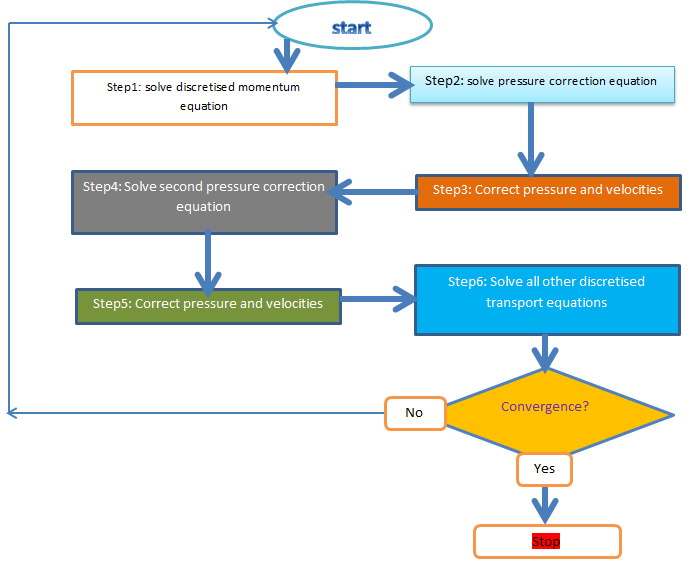
\includegraphics[width=0.85\textwidth]{Pictures/PISO.png}
%\caption{Flowchart of the PISO algorithm}
%\label{piso}
%\end{figure}

\begin{figure}[h!]
\centering % bo \centering nie wstawia dodatkowego odstępu
\usetikzlibrary{positioning}
\tikzstyle{decision} = [diamond, draw, aspect=2, text width=7em, text centered, node distance=1cm, inner sep=0pt]
\tikzstyle{block} = [rectangle, draw, text width=8em, text centered, node distance=1cm, rounded corners, minimum height=3em]
\tikzstyle{line} = [draw, -latex]
\tikzstyle{cloud} = [draw, ellipse, node distance=1cm, minimum height=3em]

\begin{tikzpicture}[node distance = 2cm, auto]
    % Place nodes
    \node [cloud] (start) {Start};
    \node [block, right=0.85cm of start] (step_one) {1: Solve the discretized momentum equation};
    \node [block, right=0.85cm of step_one] (step_two) {2: Solve the pressure correction equation};
    \node [block, right=0.85cm of step_two] (step_three) {3: Correct pressure and velocities};
    \node [block, below=1cm of step_three] (step_four) {4: Solve second pressure correction equation};
    \node [block, left=0.85cm of step_four] (step_five) {5: Correct pressure and velocities};
    \node [block, below=0.85cm of step_five] (step_six) {6: Solve all other transport equations};
    \node [decision, left=0.85cm of step_six] (convergence) {Converged?};
    \node [cloud, left=0.85cm of convergence] (stop) {Stop};
    % Draw edges
    \path [line] (start) -- (step_one);
    \path [line] (step_one) -- (step_two);
    \path [line] (step_two) -- (step_three);
    \path [line] (step_three) -- (step_four);
    \path [line] (step_four) -- (step_five);
    \path [line] (step_five) -- (step_six);
    \path [line] (step_six) -- (convergence);
    \path [line] (convergence.north) -- node {no} (step_one);
    \path [line] (convergence.west) -- node {yes} (stop);   
\end{tikzpicture}
\caption{Flowchart of the PISO algorithm}
\label{piso}
\end{figure}

%\tikzstyle{decision} = [diamond, draw, text width=10em, text centered, node distance=4cm, inner sep=0pt]
%\tikzstyle{block} = [rectangle, draw, text width=10em, text centered, node distance=4cm, rounded corners, minimum height=3em]
%\tikzstyle{line} = [draw, -latex]
%\tikzstyle{cloud} = [draw, ellipse, node distance=3cm, minimum height=3em]
%
%\begin{tikzpicture}[node distance = 2cm, auto]
%    % Place nodes
%    \node [cloud] (start) {Start};
%    \node [block, below of=start] (step_one) {1: Solve the discretized momentum equation};
%    \node [block, right of=step_one] (step_two) {2: Solve the pressure correction equation};
%    \node [block, below of=step_two] (step_three) {3: Correct pressure and velocities};
%    \node [block, left of=step_three] (step_four) {4: Solve second pressure correction equation};
%    \node [block, below of=step_four] (step_five) {5: Correct pressure and velocities};
%    \node [block, right of=step_five] (step_six) {6: Solve all other transport equations};
%    \node [decision, below of=step_five] (convergence) {Convergence?};
%    \node [cloud, below of=convergence] (stop) {Stop};
%    % Draw edges
%    \path [line] (start) -- (step_one);
%    \path [line] (step_one) -- (step_two);
%    \path [line] (step_two) -- (step_three);
%    \path [line] (step_three) -- (step_four);
%    \path [line] (step_four) -- (step_five);
%    \path [line] (step_five) -- (step_six);
%    \path [line] (step_six) |- (convergence);
%    %\path [line] (convergence) -- [near start] node {no} (step_one);
%    \path [line] (convergence) -- node {yes} (stop);   
%\end{tikzpicture}

As the flowfield resulting from the RANS analysis is averaged over time and has no distinguishable features of a turbulent flow, the DDES analysis is divided into two runs. The first run is set to create a flowfield with random flow features. This is also used for testing the convergence and data acquisition process.

Although not required by the "frozen-rotor" configuration, the timestepping is based on the rotor Blade-Pass-Frequency number. The BPF parameter is obtained by formula \ref{eq:bpf}

\begin{equation} \label{eq:bpf}
BPF = \frac{n \cdot t}{60}
\end{equation}

\noindent where $t$ is the number of blades and $n$ is the rotational speed in rpm.

For NASA R67 the base Blade Passing Frequency is equal to $5882.36 Hz$. By multiplying the BPF by four a frequency of $23529.44 Hz$ is obtained. The frequency is above the human audible range and will be used to compute the timestep. As stated in chapter \ref{approach}, in order to capture a given frequency, the timestep must be at least 4 times smaller than the period of the oscillations (equation \ref{eq:mintime}). By this approach the maximum timestep of the DDES calculation is $1.06 \cdot 10^{-5}s$. The timestep is compared with the requirements of the Courant-Friedrichs-Levy condition defined by equation \ref{eq:CFL}

\begin{equation} \label{eq:CFL}
Co = \frac{u \cdot \Delta t}{\Delta x}
\end{equation}

Considering that $u_{max} = 426.72 m/s$ and $\Delta x = 0.25 \cdot \lambda = 0.003695 m$ for desired frequency of $23529.44 Hz$ and timestep of  $1.06 \cdot 10^{-5}s$ the Courant number obtained is equal to 1.22. By rearranging the equation to solve for $\Delta t$ an equation \ref{eq:CFL2} is obtained and a calculation timestep fulfilling requirements of the CFD analysis and the direct noise formulation is computed and is equal to $8.659 \cdot 10^{-6}$.

\begin{equation} \label{eq:CFL2}
\Delta t = \frac{Co \cdot \frac{\lambda}{4}}{u_{max}}
\end{equation}

Initial timestep for the DDES analysis is set up to $5.0 \cdot 10^{-6}s$. Presented time stepping approach fulfills the Shannon-Nyquist-Whitaker theorem presented in section \ref{timestepsize}. First run was conducted for c.a. 30 thousand timesteps, during which following factors were tested: calculation efficiency dependent on the CPU core count used, data output and data format, estimated storage requirements and the output from the embedded FW-H aeroacoustical models. First run concluded, that the assumed timestep does not meet the required convergence criteria and delivered inaccurate results or flowfield with features not resembling the features characteristic for compressor flow.

The timestep was gradually decreased to a value of $1.0 \cdot 10^{-6}s$, the CPU core count was set to 120 CPU cores distributed over 5 HPC nodes. Once the first run produced a fully developed flowfield with turbulent features characteristic to the LES analysis, the case was saved and set up for a final run with full data acquisition. 

It was desired to capture at least 0.05 seconds of the flow but with some relation to geometric and operational features of the rotor. Based on the blade count and rotational speed of the rotor a time of a single periodic passage is calculated to $1.70 \cdot 10^{-4}s$. Next the required computational time is divided by the passage time to obtain the number of blade passages. 294.118 passages will occur during the 0.05s, so the number is rounded up to 295 passages and multiplied again by the passage time. Total calculation time of 0.05015 seconds is obtained. Therefore 50150 timesteps is required for full calculation runtime, with one passage being calculated in 170 timesteps.

%-----------------------------------
%	SECTION
%-----------------------------------
\section{Validation of the results}
The experimental study \citep{r67laser} provides a very extensive set of validation data for the passage flowfield. The quoted study presents results of LDA measurements of the NASA R67 compressor for relative mach number and relative flow angle at constant pitch and constant chord lines intersecting with blade span lines at 10\% intervals. Constant pitch line is derived from the blade's suction surface: 0\% percent pitch is the suction surface of one blade, 100\% pitch is the suction surface of the adjacent blade. Constant chord lines are used to plot blade-to-blade distributions of given parameters at intersection of span and constant z-coordinate surface (fig. \ref{fig_LA}).

\begin{figure}[h!]
\centering % bo \centering nie wstawia dodatkowego odstępu
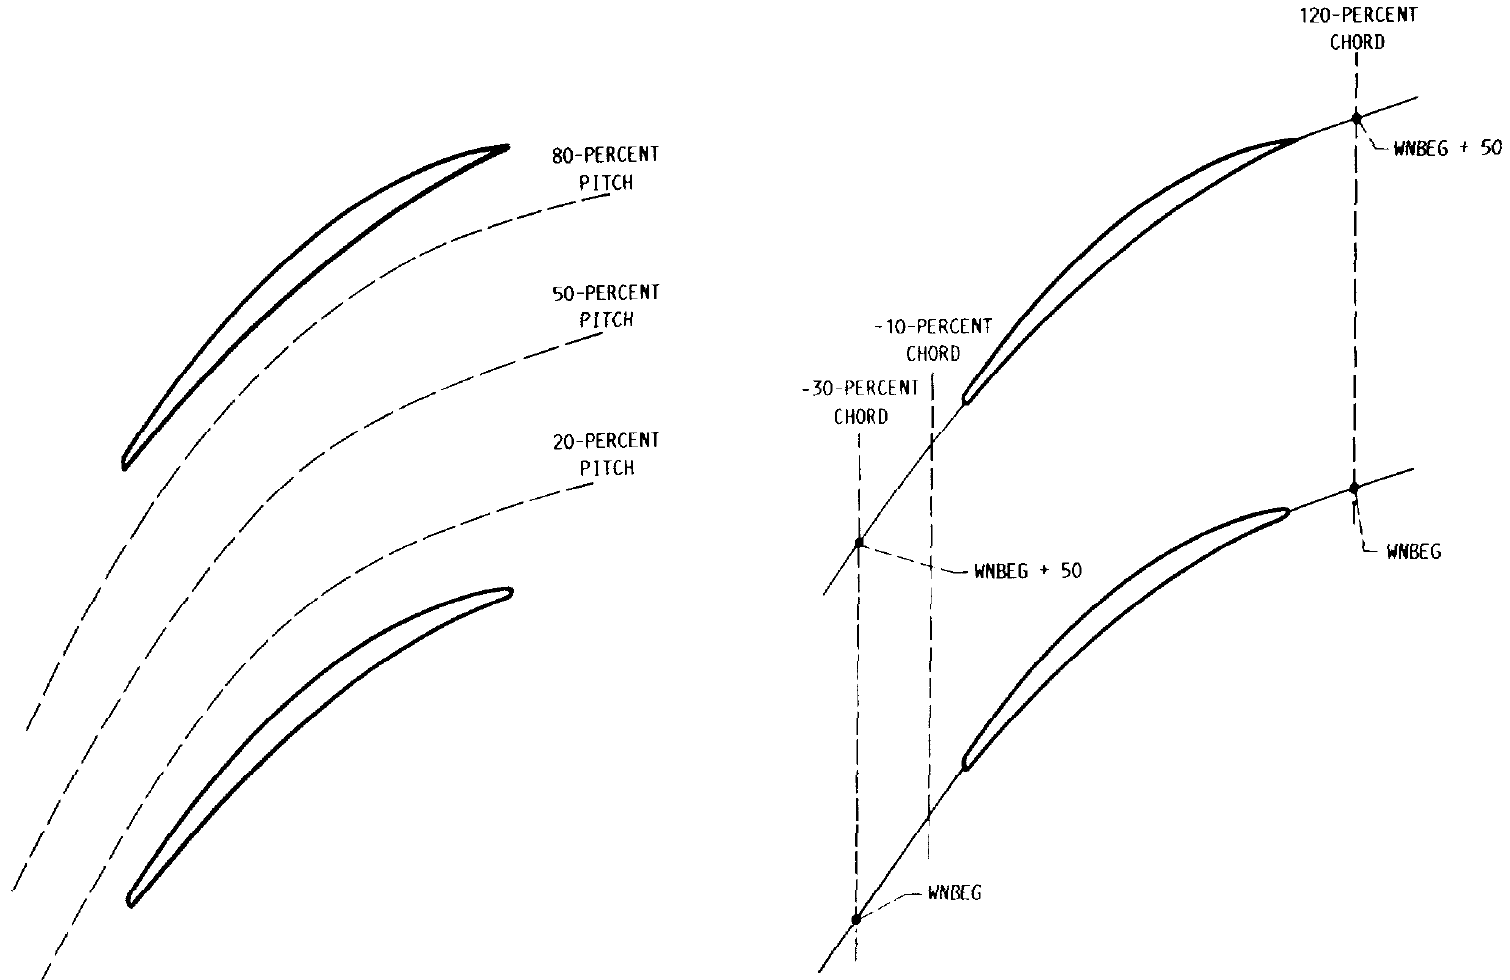
\includegraphics[width=0.85\textwidth]{Pictures/LA.png}
\caption{Schematic representation of constant pitch (left) and constant chord (right) to plot data \citep{r67laser}}
\label{fig_LA}
\end{figure}

In order to validate the CFD analysis, the constant pitch surfaces for 20\%, 50\% and 80\% constant pitch are combined with 10\%, 50\% and 90\% constant span locations, as measured from the blade tip, thus producing 9 lines to for relative Mach number and relative flow angle data. Furthermore, Mach contour plots for 10\%, 30\% and 70\% constant span surfaces (measuring from the blade tip) are compared with the experimental study.

For clarity, relative mach number plots and constant pitch plots are presented in appendix \ref{cfd_results}. 

The most simple method for validating the results is comparing the total and static pressure values on inlet and outlet boundary conditions of the domain with experimental data. Plots for static and total pressure at inlets and outlets of the domain are presented in figures \ref{pvalid_in} and \ref{pvalid_out}. 

\begin{figure}[h!]
\centering % bo \centering nie wstawia dodatkowego odstępu
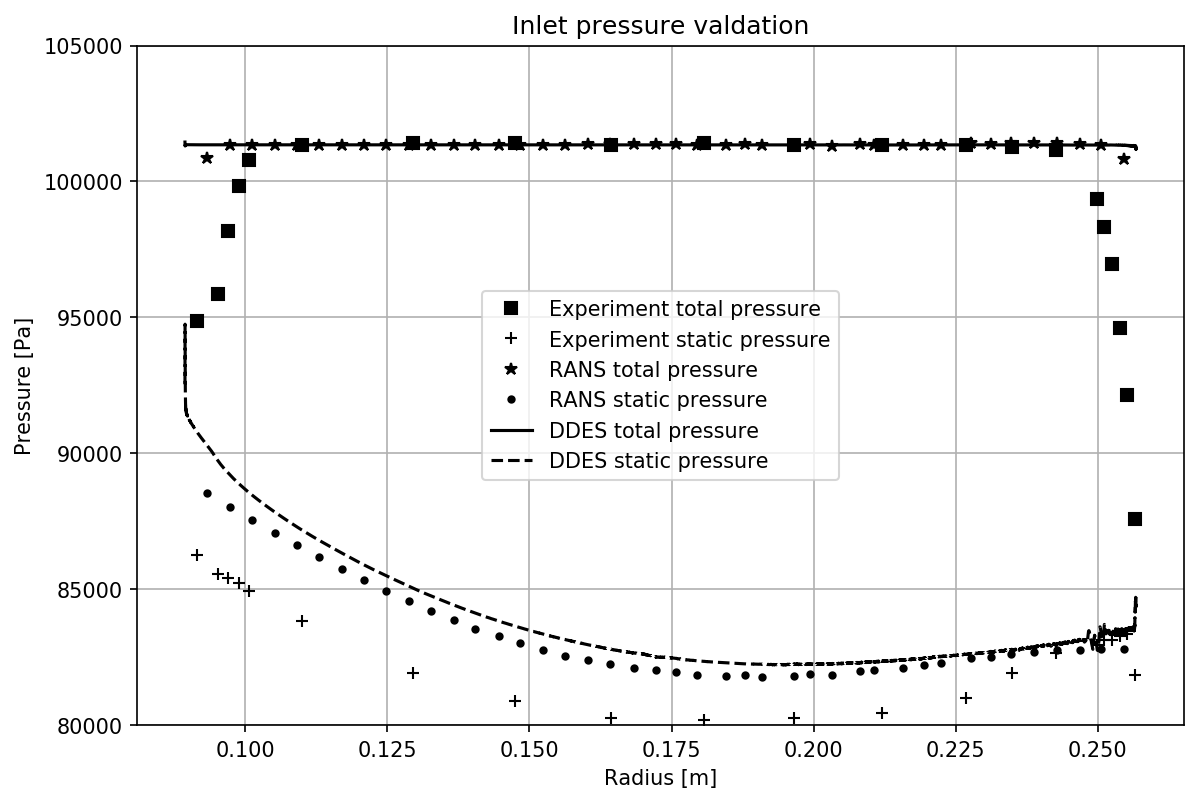
\includegraphics[width=0.8\textwidth]{Pictures/pvalid_in.png}
\caption{Inlet pressure validation}
\label{pvalid_in}
\end{figure}

\begin{figure}[h!]
\centering % bo \centering nie wstawia dodatkowego odstępu
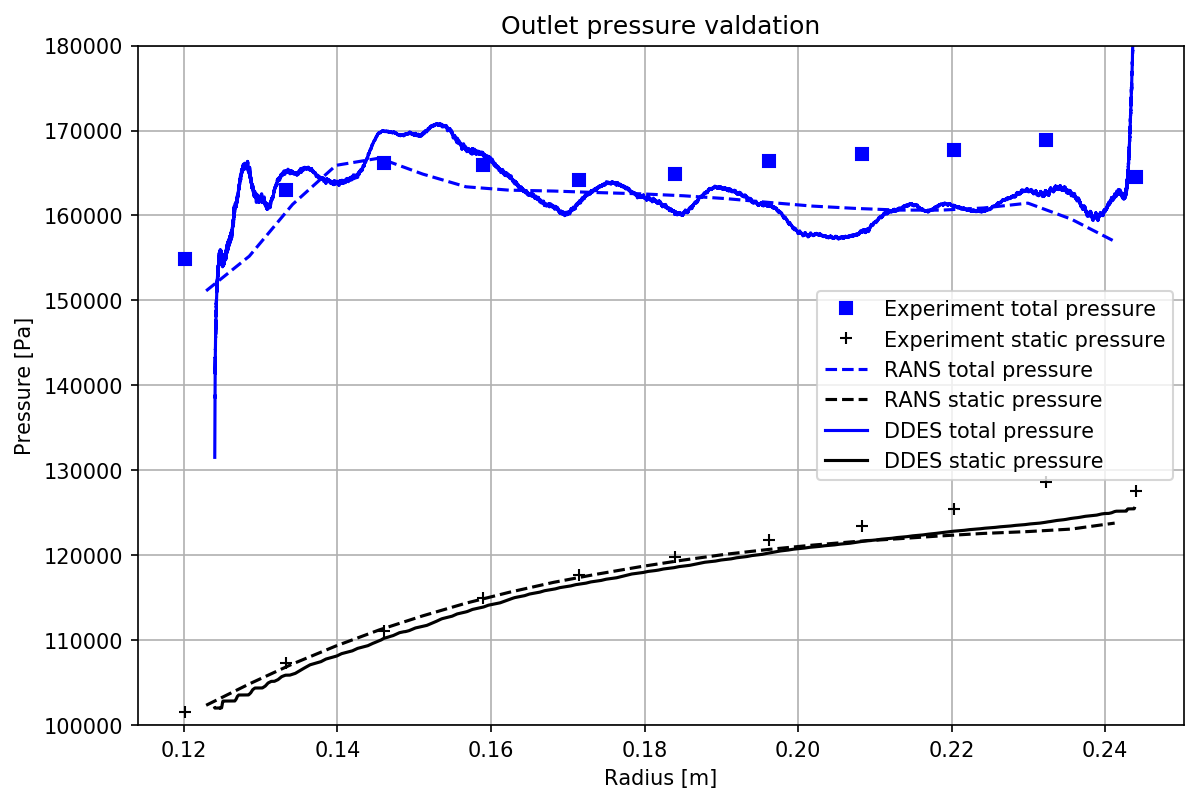
\includegraphics[width=0.8\textwidth]{Pictures/pvalid_out.png}
\caption{Outlet pressure validation}
\label{pvalid_out}
\end{figure}

%\begin{figure}[h!]
%\centering % bo \centering nie wstawia dodatkowego odstępu
%
\includegraphics[width=0.85\textwidth]{Pictures/placeholder.jpg}
%\caption{DDES analysis inlet pressure validation}
%\label{pvalid_ddes_in}
%\end{figure}
%
%\begin{figure}[h!]
%\centering % bo \centering nie wstawia dodatkowego odstępu
%
\includegraphics[width=0.85\textwidth]{Pictures/placeholder.jpg}
%\caption{DDES analysis outlet pressure validation}
%\label{pvalid_ddes_out}
%\end{figure}

Both RANS and DDES analyses produce results that are confirmed by the experimental data. Static inlet pressure plot show the discrepancy between experimental and CFD data resulting from a minor shift between the inlet and outlet CFD boundaries and the location of the pressure rake. The inlet boundary condition is moved closer towards the leading edge of the rotor, than the experimental pressure measurements array, therefore the static pressure is increased. The Mach number contour plots on the corresponding internal surfaces show the same character of the flow. Discrepancies between the experimental study and the obtained CFD results arise from a slight offset between the experimental surfaces as the mesh internal surfaces. 